% --------------------------------------------------------------------------------

\begin{exercise}[Inplementation Task: $1$-D Gridworld]

Consider the following one-dimensional \enquote{gridworld}:
You are on a route consisting of $10$ states.
The state on the left side is a terminal state with a reward of $+10$ and the state on the right is also a terminal state width a reward of $-5$.
You can move left and right.

\begin{center}
    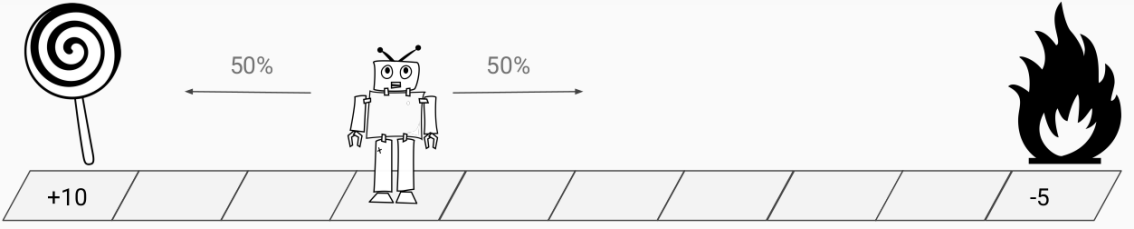
\includegraphics[width = 0.75 \textwidth]{2.24.png} \\
    $1$D Gridworld
\end{center}

Write an implementation of Dynamic Programming for estimating the values of the above states under the equiprobable random policy.

Then use policy improvement to find the optimal policy.

\end{exercise}

% --------------------------------------------------------------------------------

\begin{solution}

\phantom{}

\end{solution}

% --------------------------------------------------------------------------------
